%% ****** Start of file template.aps ****** %
%%
%%
%%   This file is part of the APS files in the REVTeX 4 distribution.
%%   Version 4.0 of REVTeX, August 2001
%%
%%
%%   Copyright (c) 2001 The American Physical Society.
%%
%%   See the REVTeX 4 README file for restrictions and more information.
%%
%
% This is a template for producing manuscripts for use with REVTEX 4.0
% Copy this file to another name and then work on that file.
% That way, you always have this original template file to use.
%
% Group addresses by affiliation; use superscriptaddress for long
% author lists, or if there are many overlapping affiliations.
% For Phys. Rev. appearance, change preprint to twocolumn.
% Choose pra, prb, prc, prd, pre, prl, prstab, or rmp for journal
%  Add 'draft' option to mark overfull boxes with black boxes
%  Add 'showpacs' option to make PACS codes appear
%  Add 'showkeys' option to make keywords appear
\documentclass[aps,preprint,superscriptaddress,endfloats*]{revtex4}
\usepackage{graphicx}
%\usepackage{hyperref}
\usepackage{subfigure}
\begin{document}

% Use the \preprint command to place your local institutional report
% number in the upper righthand corner of the title page in preprint mode.
% Multiple \preprint commands are allowed.
% Use the 'preprintnumbers' class option to override journal defaults
% to display numbers if necessary
%\preprint{}

%Title of paper
\title{Modification of the Surface Electronic and Chemical Properties of
  Pt(111) by Subsurface 3d Transition Metals}

% repeat the \author .. \affiliation  etc. as needed
% \email, \thanks, \homepage, \altaffiliation all apply to the current
% author. Explanatory text should go in the []'s, actual e-mail
% address or url should go in the {}'s for \email and \homepage.
% Please use the appropriate macro foreach each type of information

% \affiliation command applies to all authors since the last
% \affiliation command. The \affiliation command should follow the
% other information
% \affiliation can be followed by \email, \homepage, \thanks as well.
\author{J. R. Kitchin}
\affiliation{Center for Catalytic Science and Technology, Department of Chemical Engineering, University of Delaware,
  Newark, DE 19716}

\author{J. K. N{\o}rskov}
\affiliation{Center for Atomic-scale Materials Physics and Department
  of Physics, Technical University of Denmark, DK-2800 Lyngby,
  Denmark}

\author{M. A. Barteau}
\author{J. G. Chen}
\affiliation{Center for Catalytic Science and Technology, Department of Chemical Engineering, University of Delaware, Newark, DE 19716}

\date{\today}

\begin{abstract}
  The modification of the electronic and chemical properties of
  Pt(111) surfaces by subsurface 3d transition metals was studied
  using density functional theory (DFT).  In each case investigated,
  the Pt surface d-band was broadened and lowered in energy by
  interactions with the subsurface 3d metals, resulting in weaker
  dissociative adsorption energies of hydrogen and oxygen on these
  surfaces.  The magnitude of the decrease in adsorption energy was
  largest for the early 3-d transition metals and smallest for the
  late 3-d transition metals. In some cases, dissociative
  adsorption was calculated to be endothermic.  The surfaces
  investigated in this study had no lateral strain in them,
  demonstrating that strain is not a necessary factor in the
  modification of bimetallic surface properties.  The implications of
  these findings are discussed in the context of catalyst design,
  particularly for fuel cell electrocatalysts.
\end{abstract}

% insert suggested PACS numbers in braces on next line
\pacs{}
% insert suggested keywords - APS authors don't need to do this
\keywords{Bimetallic, Pt, ligand effect, DFT}

%\maketitle must follow title, authors, abstract, \pacs, and \keywords
\maketitle

\section{Introduction}
Pt-group metals are among the most widely used catalysts.  They are
also, however, among the most expensive metals.  Thus, there is a
particular interest in modifying the chemical properties of less
expensive metals to mimic the Pt-group metals, or alternatively,
modifying the properties of Pt to achieve higher activity or
selectivity in a catalytic reaction so that less metal would be
required.  For example, in hydrogen fuel cell applications one needs
an anode electrocatalyst that is both CO-tolerant and efficient at
splitting hydrogen. Likewise, the cathode electrocatalyst must be efficient at
splitting oxygen, but not poisoned by the O-containing products.
Bimetallic catalysts represent one approach to meeting these criteria, as
the adsorption properties of molecules can be tuned by the composition
and structure of the bimetallic surface \cite{sinfelt1983}.  However, it is
still difficult to know a priori how the chemical and electronic
properties of a particular bimetallic surface will be modified
relative to the parent metals.  These properties depend explicitly on
the geometric structure and chemical composition of the surfaces
considered.

The adsorption properties of many atoms and small molecules on
transition metals have been shown by Hammer and N{\o}rskov to depend
primarily on the electronic structure of the surface
\cite{hammer1995:_elect,hammer2000:_adv_cat}, which in turn is
determined its geometric structure and chemical composition.  In that
work it was shown that the interactions between adsorbates and
transition metal surfaces could be considered via a two level orbital
mixing picture.  The adsorbate orbitals are first broadened by
interactions with the broad s-electron band, and then split by strong
interactions with the sharper d-band.  These authors further
demonstrated that modification of the surface electronic structure can
result in a predictable modification of the surface chemical
properties, for example the adsorption properties of small molecules.
Specifically, a correlation between the average energy of the d-band
and the adsorption energy of many atoms and small molecules was
established.

There are two critical factors that contribute to the modification of
the electronic properties of a metal in a bimetallic surface.  First,
the surface bond lengths are typically different than those of the
parent metals.  This gives rise to strain effects that modify the
electronic structure of the metal through changes in orbital overlap
\cite{mavrikakis1998:_effec_strain_metal}.  According to these
arguments, when the surface atoms are subjected to tensile strain, the
d-orbital overlap is decreased, resulting in a sharpening of the
d-band and an upshift in its average energy (the d-band center).  For
simple adsorbates such as H, O and CO, this results in a stronger
adsorption energy when compared to those of the parent metal surface.
On the other hand, when the surface atoms are under compressive
strain, the d-orbital overlaps are increased, resulting in a
broadening of the d-band and a lowering of its average energy.
Correspondingly, the adsorption energies of simple adsorbates are
expected to decrease compared to those of the parent metal surface.

The second factor that contributes to the modification of surface
properties in bimetallic systems is the electronic interaction between
the two metals.  This effect, also termed the ligand effect
\cite{liu2001:_ligan,gauthier2001:_adsor_co}, arises because the
presence of other metals around a metal atom changes its electronic
environment, giving rise to modifications of its electronic structure
and consequently, its chemical properties.  A critical question is
which of these two effects, strain or the ligand effect, is more
important?  More specifically, under what conditions does strain
dominate the modification of behavior of bimetallic surface
properties, and under what conditions does the ligand effect dominate?
The purpose of the present paper is to identify conditions where the
ligand effect can have a dominant role in the modification of the
chemical properties of a bimetallic surface.  In this respect, it is
complementary to the previous work that identified the importance of
strain in the modification of the electronic and chemical properties
of bimetallic surfaces \cite{mavrikakis1998:_effec_strain_metal} and
seeks to further our understanding of how to design these surfaces.
There are also other important phenomena that can affect the
properties of bimetallic surfaces, such as ensemble effects
\cite{liu2001:_ligan}, and bifunctional catalysis, in which the two
metals function independently. These phenomena were not considered in
this work.
 
Ruban et al. studied the changes in the electronic structure of
epitaxial monolayers of one metal on another metal for the late
transition metals \cite{ruban1997:_surfac}.  In that work, the changes
in electronic structure were largely attributed to the strain induced
by epitaxy.  However, it is difficult to separate the effect of strain
from that of the ligand effect in this scenario, because they both
exist simultaneously.  On the other hand, the fact that these authors
were able to account for the changes so well using strain alone
suggests that the ligand effect may be weak in these systems.

The cleanest way to single out the ligand effect is by using an
epitaxial subsurface layer in an otherwise unperturbed surface, so
that the surface lattice constant is not changed.  In this scenario,
the subsurface atoms will be strained, as they must adopt the lattice
constant of the surface, but the surface will not be laterally
strained.  Therefore, any changes in the electronic or chemical
properties of the surface may be considered as primarily due to the
interactions with the subsurface metal atoms (the ligand effect) and
not to surface strain.  Thus, in this study we examine Pt(111) slabs,
where the second layer of metal atoms has been replaced by one of the
3d transition metals.

Some explanation of why this is a reasonable and relevant model is
needed.  Pt segregates to the surface in many Pt-bimetallic mixtures,
and a Pt-rich surface is expected in all of the cases in the present
study (for close-packed fcc (111) surfaces) \cite{ruban1999}.
Additionally, there are several reported cases of Pt alloys where the
first layer is Pt-rich, and the second layer is enriched in the other
metal, most notably Ni/Pt(111) alloys \cite{gauthier1985}.  Kitchin et
al. recently reported experimental investigations of the effects of
subsurface Ni on the chemical properties of Pt(111) single crystals
\cite{kitchin2003:_elucid_ni_pt}. In that study, thin films of Ni on
Pt(111) were prepared by physical vapor deposition of Ni onto the
surface, followed by subsequent annealing to drive the Ni atoms into
subsurface positions.  This particular structure was found to have a
weaker hydrogen adsorption energy than either pure Ni(111) or Pt(111)
surfaces.  Several other investigations of Pt-3d alloys in fuel cell
applications have suggested that the alloy films used in these studies
were covered by a Pt skin \cite{toda1999,watanabe2000,wan2002}. Thus,
our model is an idealization of Pt-rich Pt-3d alloy surfaces intended to
illustrate the electronic interactions between the surface atoms and
subsurface atoms in the absence of strain.

We did not consider the possibility that the formation of a bulk alloy
could change the lattice constant of the slab, but the effect of this
could be estimated from the principles of strain
\cite{mavrikakis1998:_effec_strain_metal} and is discussed later.  We
also did not consider the stability of these structures with respect
to reconstructions or in the presence of adsorbates.  Oxygen is
reported to induce Ni segregation in Ni/Pt alloys \cite{weigand1992},
and the oxidation of Pt$_3$Ti surfaces at low oxygen pressures is also
reported \cite{bardi1984}.  Toda et al. have reported, however, that
in many of the Pt-3d systems they have investigated that the alloy
particles are covered by a thin skin of Pt, even under hot H$_3$PO$_4$
reaction conditions and in the electrocatalytic reduction of O$_2$
\cite{toda1999}.  Clearly, there are non-trivial issues to be
understood on the effects of surface segregation under reaction
conditions, but this topic is beyond the scope of this paper.

\section{Calculation Details}
The Pt(111) surfaces were modeled by a 2$\times$2 unit cell with four
layers of metal atoms periodically repeated with 4-6 equivalent layers
of vacuum ( $>$ 10 \AA ) separating the slabs to represent the Pt(111)
surface.  The four atoms in the second layer of the slab were
substituted with one of the 3d transition metals between (and
including) Ti and Ni.  The first and second layers were allowed to
relax to their lowest energy configuration, whereas the third and
fourth layers were frozen at the bulk Pt-Pt distance (2.84 \AA, as
determined by DFT for the RPBE exchange/correlation functional used in
this work).  The electronic structure was calculated with the
Dacapo-2.7 code \cite{campos}, which uses plane waves as the basis
set, and ultra-soft Vanderbilt pseudopotentials (created with the PW91
exchange/correlation functional) to represent the core electrons.  The
mismatch between the exchange/correlation functional used to create
the pseudopotentials and the the exchange/correlation functional used
in the calculations is not expected to affect the results
\cite{hammer1999:_improv_pbe}. In all of the calculations, a $4\times
4\times 1$ Monkhorst-Pack k-point set was used. For the H adsorption
calculations a plane wave cutoff energy of 350 eV was used, and for
the O adsorption calculations a 450 eV plane wave energy cutoff was
used. The calculated adsorption energies on Pt changed by less than
0.05 eV with higher cutoff energies.  Maximum symmetry constraints
were applied in all cases.  In previous work on Ni/Pt systems, it was
found that including spin polarization in the calculations did not
affect the trends in adsorption energies observed
\cite{kitchin2003:_elucid_ni_pt}.  Therefore, spin polarization was
not included in any of the calculations in this work.  A dipole
correction scheme was used to ensure the slabs were electronically
decoupled.  The d-band density of states was determined by projection
of the plane waves onto spherical harmonic orbitals, with the cutoff
radius at infinity.  The d-band center was calculated as the first
moment of the projected d-band density of states on the surface atoms
referenced to the Fermi level, and the mean squared d-band width was
calculated as the second moment.

The structure of the surface d-electron bands is a critical factor in
the adsorption properties of many simple adsorbates
\cite{hammer2000:_adv_cat}.  In correlating adsorption properties with
the d-band structure, it is convenient to use a single, characteristic
value that is representative of the d-band.  The density of states at
the Fermi Level, $\rho_F$, has been used in many studies because the
electrons at the Fermi level are the most energetically available
electrons for chemical reaction. The value of $\rho_F$, however, is
only a single point in the distribution of states, and may reflect
little of the d-band structure.  Furthermore, there has been only
limited success in understanding trends in catalysis using $\rho_F$
\cite[Ch. 2]{vansanten1991}.  In some cases, however, there is a
general correlation between $\rho_F$ and the d-band properties, as
will be shown later.  Another choice of parameter for correlation has
been the number of d-holes, or unoccupied d-states.  The reasoning is
that these empty orbitals are required to interact with the occupied
states in adsorbates.  It will become apparent below why this
parameter is unsuitable to explain the variations in dissociative
adsorption energies of H$_2$ and O$_2$ for the systems examined in
this work.

Hammer and N{\o}rskov have shown that the interactions between
adsorbates and transition metal surfaces involve the entire d-band
\cite{hammer2000:_adv_cat}.  Therefore, a more logical choice of
parameters is one that depends in a functional way on the entire
d-band, such as its average energy.  The first moment of the d-band is
the average energy of the band, also called the d-band center.  An
alternative choice would be the mean squared band width, or the second
moment.  As we will show later, however, these two moments are highly
correlated in these systems.

\section{Results and Discussion}
\subsection{Electronic Structure}
The results of our electronic structure calculations are listed in
Table \ref{tab1} and are shown graphically in Figure \ref{fig1}.  In
each bimetallic case, the surface Pt d-band is lower in energy and
broader in width than the pure Pt slab.  The magnitude of the shift in
the surface d-band center relative to pure Pt(111) generally increases as the
subsurface metal moves to the left in the periodic table, consistent
with the trend in the magnitude of the matrix element \cite{ruban1997:_surfac} for
these metals.  This suggests why strain was capable of explaining
the trends shown by Ruban et al. \cite{ruban1997:_surfac}; the ligand effect is
weakest between the late transition metals, and most likely to be
dominated by strain for these bimetallic combinations.  Interactions
between early transition metals and late transition metals are seen to
be the strongest, and these combinations were not considered in that
work.
  
\begin{table}%[H] add [H] placement to break table across pages
\caption{\label{tab1}Electronic and geometric structure calculation results.}
\begin{ruledtabular}
\begin{tabular}{ccccc}
\hline
Second & d-band & mean squared  & d-band & layer\\
layer  & center &  d-band width & filling & separation\\
identity & (eV) & (eV$^2$) & (electrons/atom) & (\AA) \\\hline
Ti & -3.16 & 13.03 & 9.35 & 2.14 \\\hline
V & -3.18 & 13.21 & 9.32 & 2.10  \\\hline
Cr & -3.12 & 12.84 & 9.30 & 2.04 \\\hline
Mn & -3.00 & 12.14 & 9.29 & 2.01 \\\hline
Fe & -2.84 & 11.10 & 9.29 & 2.05 \\\hline
Co & -2.74 & 10.47 & 9.30 & 2.04 \\\hline
Ni & -2.60 & 9.70 & 9.31 & 2.04 \\\hline
Pt & -2.44 & 9.11 & 9.26 & 2.34 \\\hline
\end{tabular}
\end{ruledtabular}
\end{table}

\begin{figure*}
\subfigure%
{
\label{fig1a}
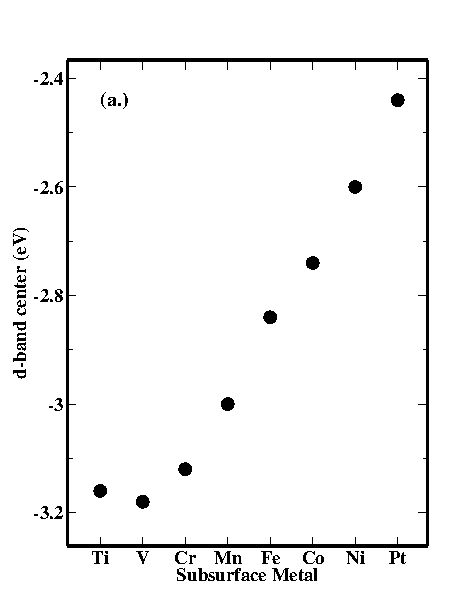
\includegraphics{figures/figure_1a}
}
\hspace{0cm}
\subfigure{
\label{fig1b}
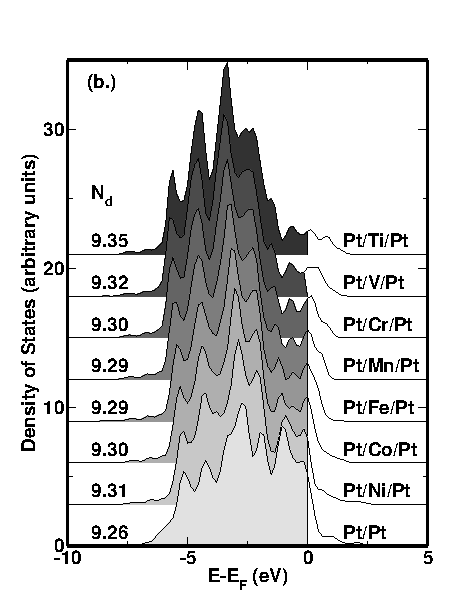
\includegraphics{figures/figure_1b}}
\caption{a. Variations in the surface d-band center of Pt(111) slabs
  containing subsurface 3d metals. b. Calculated surface d-band DOS for
  subsurface-3d-metal-containing Pt slabs.  The number of
  d-electrons/surface atom is shown for each band.\label{fig1}}
\end{figure*}

The number of d-electrons per surface Pt atom was calculated by
integrating the projected surface d-band density of states up to the
Fermi level.  In each case, we calculated approximately 9.3
d-electrons/Pt atom (also shown in Table \ref{tab1} and Figure
\ref{fig1b}.).  Thus, the d-band filling does not appear to change
substantially by the formation of the bimetallic structure.
Correspondingly, the number of unoccupied d-states does not change
either. Thus, correlations between the number of d-holes and chemical
properties of these systems are not expected.  

Conservation of the d-band filling is significant, because it means
that if the band widens, it must move down in energy in order to
maintain the constant d-band occupancy.  Conversely, if the band becomes
narrower, it must move up in energy to conserve the d-band filling.
Thus, the band width and band center are related.  This can be shown
analytically, by assuming a simple, rectangular form of
the d-band.  By assuming that the d-band filling is a constant (as
observed in our DFT calculations) and using the constraint that the
total number of states is conserved, one can easily show that the
second moment of the band, the mean squared band width
($\overline{W}$), is proportional to the square of the first moment of
the band, the d-band center ($\epsilon_d$),
\begin{equation}\label{eq1}
\overline{W} = \frac{1}{3}\biggl(\frac{1}{0.5 -f_d} \epsilon_d\biggr)^2(1-3f_d+3f_d^2)
\end{equation}
where $f_d$ is the fractional filling of the d-band, and is a
constant.  The calculated surface d-band density of states are not
rectangular in shape (see Figure \ref{fig1b}), but the same
constraints apply to them and this functional relationship still holds
true, as shown in Figure \ref{fig2a}, where $\sqrt{\overline{W}}$ is
seen to vary linearly with $\epsilon_d$ with a negative slope as
predicted by Eq.  (\ref{eq1}) for $f_d=0.93$.

\begin{figure*}
\subfigure%
{
\label{fig2a}
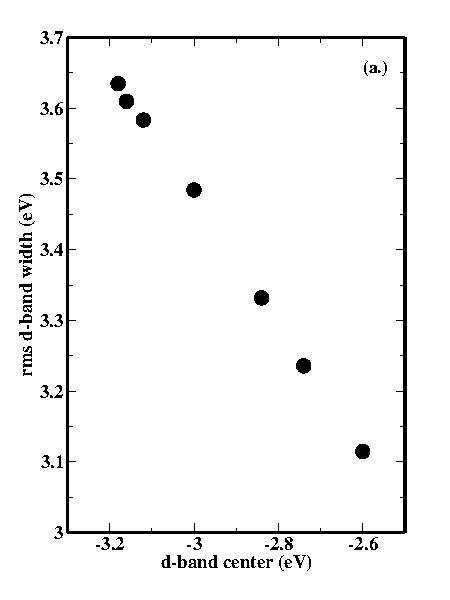
\includegraphics{figures/figure2a}
}
\hspace{0cm}
\subfigure{
\label{fig2b}
\includegraphics{figures/figure2b}}
\caption{\label{fig2}
  a) Correlation between the first and second moments of the d-band
  density of states. b) Correlation between the density of states at
  the Fermi level and the d-band center for the total density of
  states and d-band density of states.}
\end{figure*}

Since the height of the rectangle must decrease as the bands broaden
to maintain a constant total number of states (constant area), the
rectangular band model predicts that the density of states at the
Fermi level should decrease as the band gets wider.  Figure
\ref{fig2b} shows that the density of states at the Fermi level
generally decreases with decreasing energy of the d-band center, for
both the d-band and the total density of states, as predicted by the
rectangular band model.  Careful inspection of Figure \ref{fig1b}
reveals that the decrease in the density of states at the Fermi level
arises from the combination of a state crossing the Fermi level and
the diminution of that state.  Therefore, unlike the d-band center,
which is a function of all the states in the d-band, the density of
states at the Fermi level may depend sensitively on the behavior of a
localised state near the Fermi level. However, bonding interactions
between the d-band and an adsorbate depend on the nature of the entire
d-band, not just the behavior of a single state.  Consequently, the
density of states at the Fermi level is not generally expected to be a
useful indicator of chemical reactivity.

The electronic properties of the surface Pt atoms in these
calculations are modified without the introduction of lateral surface
strain.  The modification is due primarily to the electronic
interactions between the Pt surface atoms and the second layer 3d
metal atoms.  Within a tight-binding formalism, the d-band width is
proportional to the matrix elements between the d-orbitals
\cite{harrison1989}. For an alloy consisting of metal 1 and metal 2,
these can be estimated by
\begin{equation}
V_{ddm}^{(1,2)}=\eta_{ddm} \frac{\hbar^2(r_d^{(1)}r_d^{(2)})^{3/2}}{md^5}
\end{equation}
where $\eta_{ddm}$ is a constant, set to unity for convenience,
$\hbar^2/m=7.62$ eV\AA$^2$.  $r_d^{(i)}$ is a length characteristic of
metal $i$, and can be found in the Solid State Table in Reference
\citealp{harrison1989}. Finally, $d$ is the distance separating the
metals, the interlayer separation found in Table \ref{tab1}.  These
matrix elements are related to the strength of the interaction
(bonding) between the two metals; in this work that is the strength of
the interaction between the surface Pt atoms and the subsurface 3d
metal.  The proportionality between the Pt-X matrix element and the
root mean squared (rms) width of the surface Pt with subsurface metal
X is shown in Figure \ref{fig:V:width}. Clearly the surface d-band
width is proportional to the matrix element between the surface Pt and
subsurface metal, suggesting that the change in band width is due to
strong bonding between the Pt and subsurface 3d metal. As discussed
earlier, the band then moves down in energy to conserve the number of
d-states.

\begin{figure}
\includegraphics{figures/figure3}
\caption{Relationship between the surface d-band width of Pt with
  subsurface metal X and the matrix element between Pt-X.}
\label{fig:V:width}
\end{figure}

Finally, we consider the effect that the lattice constant could change
due to formation of a Pt-3d alloy. The nearest neighbor distances for
all the 3d transition metals except Ti are smaller than that of Pt. In
the context of Vegard's law, which predicts a linear variation in
alloy lattice constant with composition, this means that the lattice
constant of the alloy will be smaller than that of Pt.  According to
the strain arguments discussed earlier, this indicates that the d-band
will likely be even wider and lower in energy than shown here in this
work.  Thus, assuming that the alloys would still have an fcc-like
structure, the estimates above could be viewed as an upper bound on
the alloy results.  The real alloys are certain to be much more
complicated than these simple models though. Some of the 3d metals
have bcc crystal structures, others have hcp structures, and the
variations in lattice constant with composition are usually not linear
\cite{gschneidner1962:_depar_law}.  A change in the alloy crystal
structure would have a corresponding change in electronic and chemical
properties, but this is beyond the scope of this paper.

\subsection{H$_2$ and O$_2$ Dissociative Adsorption Energies}
In addition to characterizing the electronic structure of these slabs,
we have also calculated the dissociative adsorption energies for H$_2$
and O$_2$ on each slab.  The energetics of dissociative adsorption of
these molecules and their subsequent surface reactions play an
important role at the surfaces of fuel cell electrocatalysts
\cite{markovic2002:_surfac_scien}.  If oxygen binds too strongly to
the cathode, for example, it could poison the surface and reduce its
activity.  On the other hand, if it binds too weakly, the coverage of
O adatoms may be too low for significant reaction to take place or
dissociation could become activated.
%
Dissociative adsorption energies were calculated as \(2 E_{slab,ads}-2
E_{slab} -E_{molecule}\), where $E_{slab,ads}$ is the energy of a slab
with an O or H atom on it at 0.25 monolayer coverage in the
three-fold, fcc site. $E_{slab}$ is the energy of a clean slab, and
$E_{molecule}$ is the energy of an H$_2$ or O$_2$ molecule in the gas
phase. Zero-point energies were not included in any of the
calculations.  As with the clean slabs, the top two layers and the
adsorbate were allowed to relax to the lowest energy configuration.
The third and fourth layers were fixed at the bulk lattice parameter
previously mentioned, 2.84 \AA.  The results are summarized in Figure
\ref{fig4}.  There is a nearly linear trend in the adsorption energies
versus the surface d-band center; the adsorption energy decreases as
the d-band center becomes more negative.  The dissociative adsorption
for both H$_2$ and O$_2$ becomes endothermic when the surface d-band
center shifts to sufficiently negative values. It is now obvious why
the density of states at the Fermi level has sometimes been
successfully used in correlations with chemical properties; in some
cases, there is a strong correlation between the d-band center and the
density of states at the Fermi level (see Figure \ref{fig2b}).
However, it is also apparent in Figure \ref{fig2b} that the
correlation is not monotonic, and thus may be non-trivial to use.
Therefore, the d-band center with the more intuitive adsorption model
of Hammer and N{\o}rskov is a more useful indicator of chemical
reactivity.

\begin{figure*}
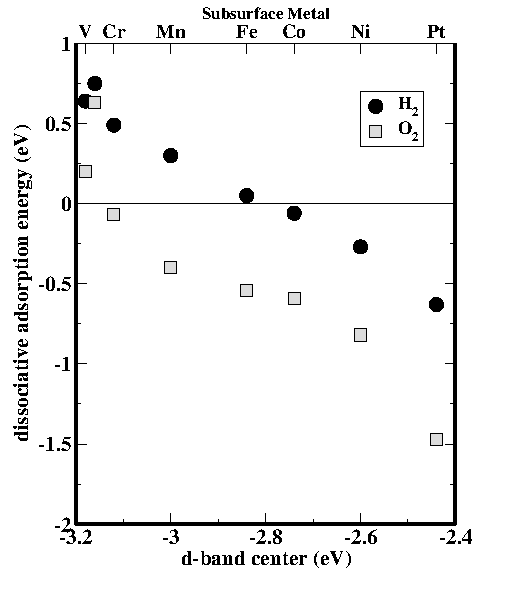
\includegraphics{figures/figure4}%
\caption{\label{fig4}
  Trends in dissociative adsorption energies for H$_2$ and O$_2$ on
  Pt(111) slabs containing subsurface 3d metals. }
\end{figure*}

These results have important implications for catalyst design,
particularly for proton exchange membrane (PEM) fuel cell
electrocatalysts.  On the PEM fuel cell anode, one desires a catalyst
that is both CO tolerant and active at dissociating H$_2$.  The CO
tolerance of a surface can be enhanced by modifying it in such a way
that CO binds more weakly to it, thus reducing its coverage.  One
method for reducing the CO adsorption energy on a surface is to lower
its d-band center, by alloying with another metal, for example
\cite{hammer1996:_co}.  The present work shows, however, that if the surface
d-band center is lowered too much, then dissociative adsorption of
H$_2$ becomes energetically unfavorable.  Thus, the bimetallic surface
may be very CO-tolerant, but unsuitable for use as a fuel cell anode
catalyst.

For the cathode, a similar balance must be made.  One needs a catalyst
that can dissociate O$_2$, but not bind the resulting O adatoms too
tightly.  Enhanced electrocatalytic activity in the reduction of
oxygen was shown on several Pt-3d alloy surfaces, particularly Pt-Fe
and Pt-Ni, compared to that of pure Pt \cite{toda1999}.  In that work,
Toda et al.  suggest that adsorption of O$_2$ is the rate-determining
step, and that alloying results in an enhanced metal-oxygen
interaction that leads to an increased coverage of O$_2^-$, which
subsequently dissociates.  However, it has been shown that reducing
the dissociative adsorption energy of oxygen results in an increase in
the oxygen dissociation barrier \cite{norskov2002:_univer}.
Therefore, it seems likely that the dissociation barrier for O$_2$ on
the Pt-3d surfaces in this study would be higher than that on pure
Pt(111).  On the other hand, a more weakly bound O adatom may be more
reactive than a more strongly bound O adatom, resulting in a rate
enhancement.  Finally, the adsorption energies of both H$_2$ and O$_2$
decrease on these bimetallic surfaces due to the downshift in energy
of the surface d-band center.  Markovi\'c et al. report that the
enhancements in the oxygen reduction reaction on Pt$_3$Co and Pt$_3$Ni
surfaces can be explained by a reduction in the surface coverage of
OH$_{ads}$ species \cite{markovic2001:_oxygen_pt_pt}. The adsorption
energy of many atomic adsorbates and small molecules decreases as the
surface d-band center decreases in energy \cite{norskov2002:_univer}.
It is probable that the adsorption energies of surface species such as
OH$_{ads}$ will decrease as well, which could result in a lower
coverage of these species on the surface and more available active
sites for oxygen dissociation.

\section{Conclusions}
In the present study we have shown how subsurface 3d transition metal
atoms modify the electronic and chemical properties of a Pt surface by
the ligand effect in the absence of lateral strain.  In each case, the
Pt surface d-band was broadened by the interactions with the
subsurface 3d metal, with the magnitude of the effect increasing as
the subsurface 3d metal changed from Ni to Ti. The number of
d-electrons remained constant in each case, and consequently the
average energy of the band (the d-band center) decreased to maintain a
constant d-band filling, in accordance with a rectangular band model.
A simple model relating the d-band width to the matrix element between
the surface Pt and subsurface 3d metal was introduced to explain the
change in width.  The decrease in the average energy of the surface
d-band caused a corresponding decrease in the dissociative adsorption
energies of H$_2$ and O$_2$, in some cases making dissociative
adsorption endothermic.  These results show the importance of the
ligand effect in the chemical properties of bimetallic surfaces
containing both early and late transition metals.  This work further
demonstrates that adsorption properties of molecules on transition
metal surfaces can be tuned by changes in the surface d-band
structure, either by strain-induced shifts or through the ligand
effect.

 
% If you have acknowledgments, this puts in the proper section head.
\begin{acknowledgments}
This work was funded in part by Basic Energy Sciences, Department of
Energy (Grant DE-FG02-04ER15501).  JRK acknowledges the National
Science Foundation Graduate Research Fellowship program.  The Center
for Atomic-scale Materials Physics is sponsored by the Danish National
Research Foundation. The DFT calculations have been performed with
support from the Danish Center for Scientific Computing through grant
no. HDW-1101-05.
\end{acknowledgments}

% Create the reference section using BibTeX:
\bibliography{Pt3d_version2-bib}

\end{document}
%
% ****** End of file template.aps ******

